\section{Impact of Detection on Tracking Performance}
\label{sec:results/section_c}

To analyze how much the detection performance impacts the tracking performance, MOTA is plotted against mAP-50 across all video sequences for "all" object classes as shown in Figure \ref{fig:MOTA_vs_mAP50}.
\begin{figure}[!tb]
  \centering
  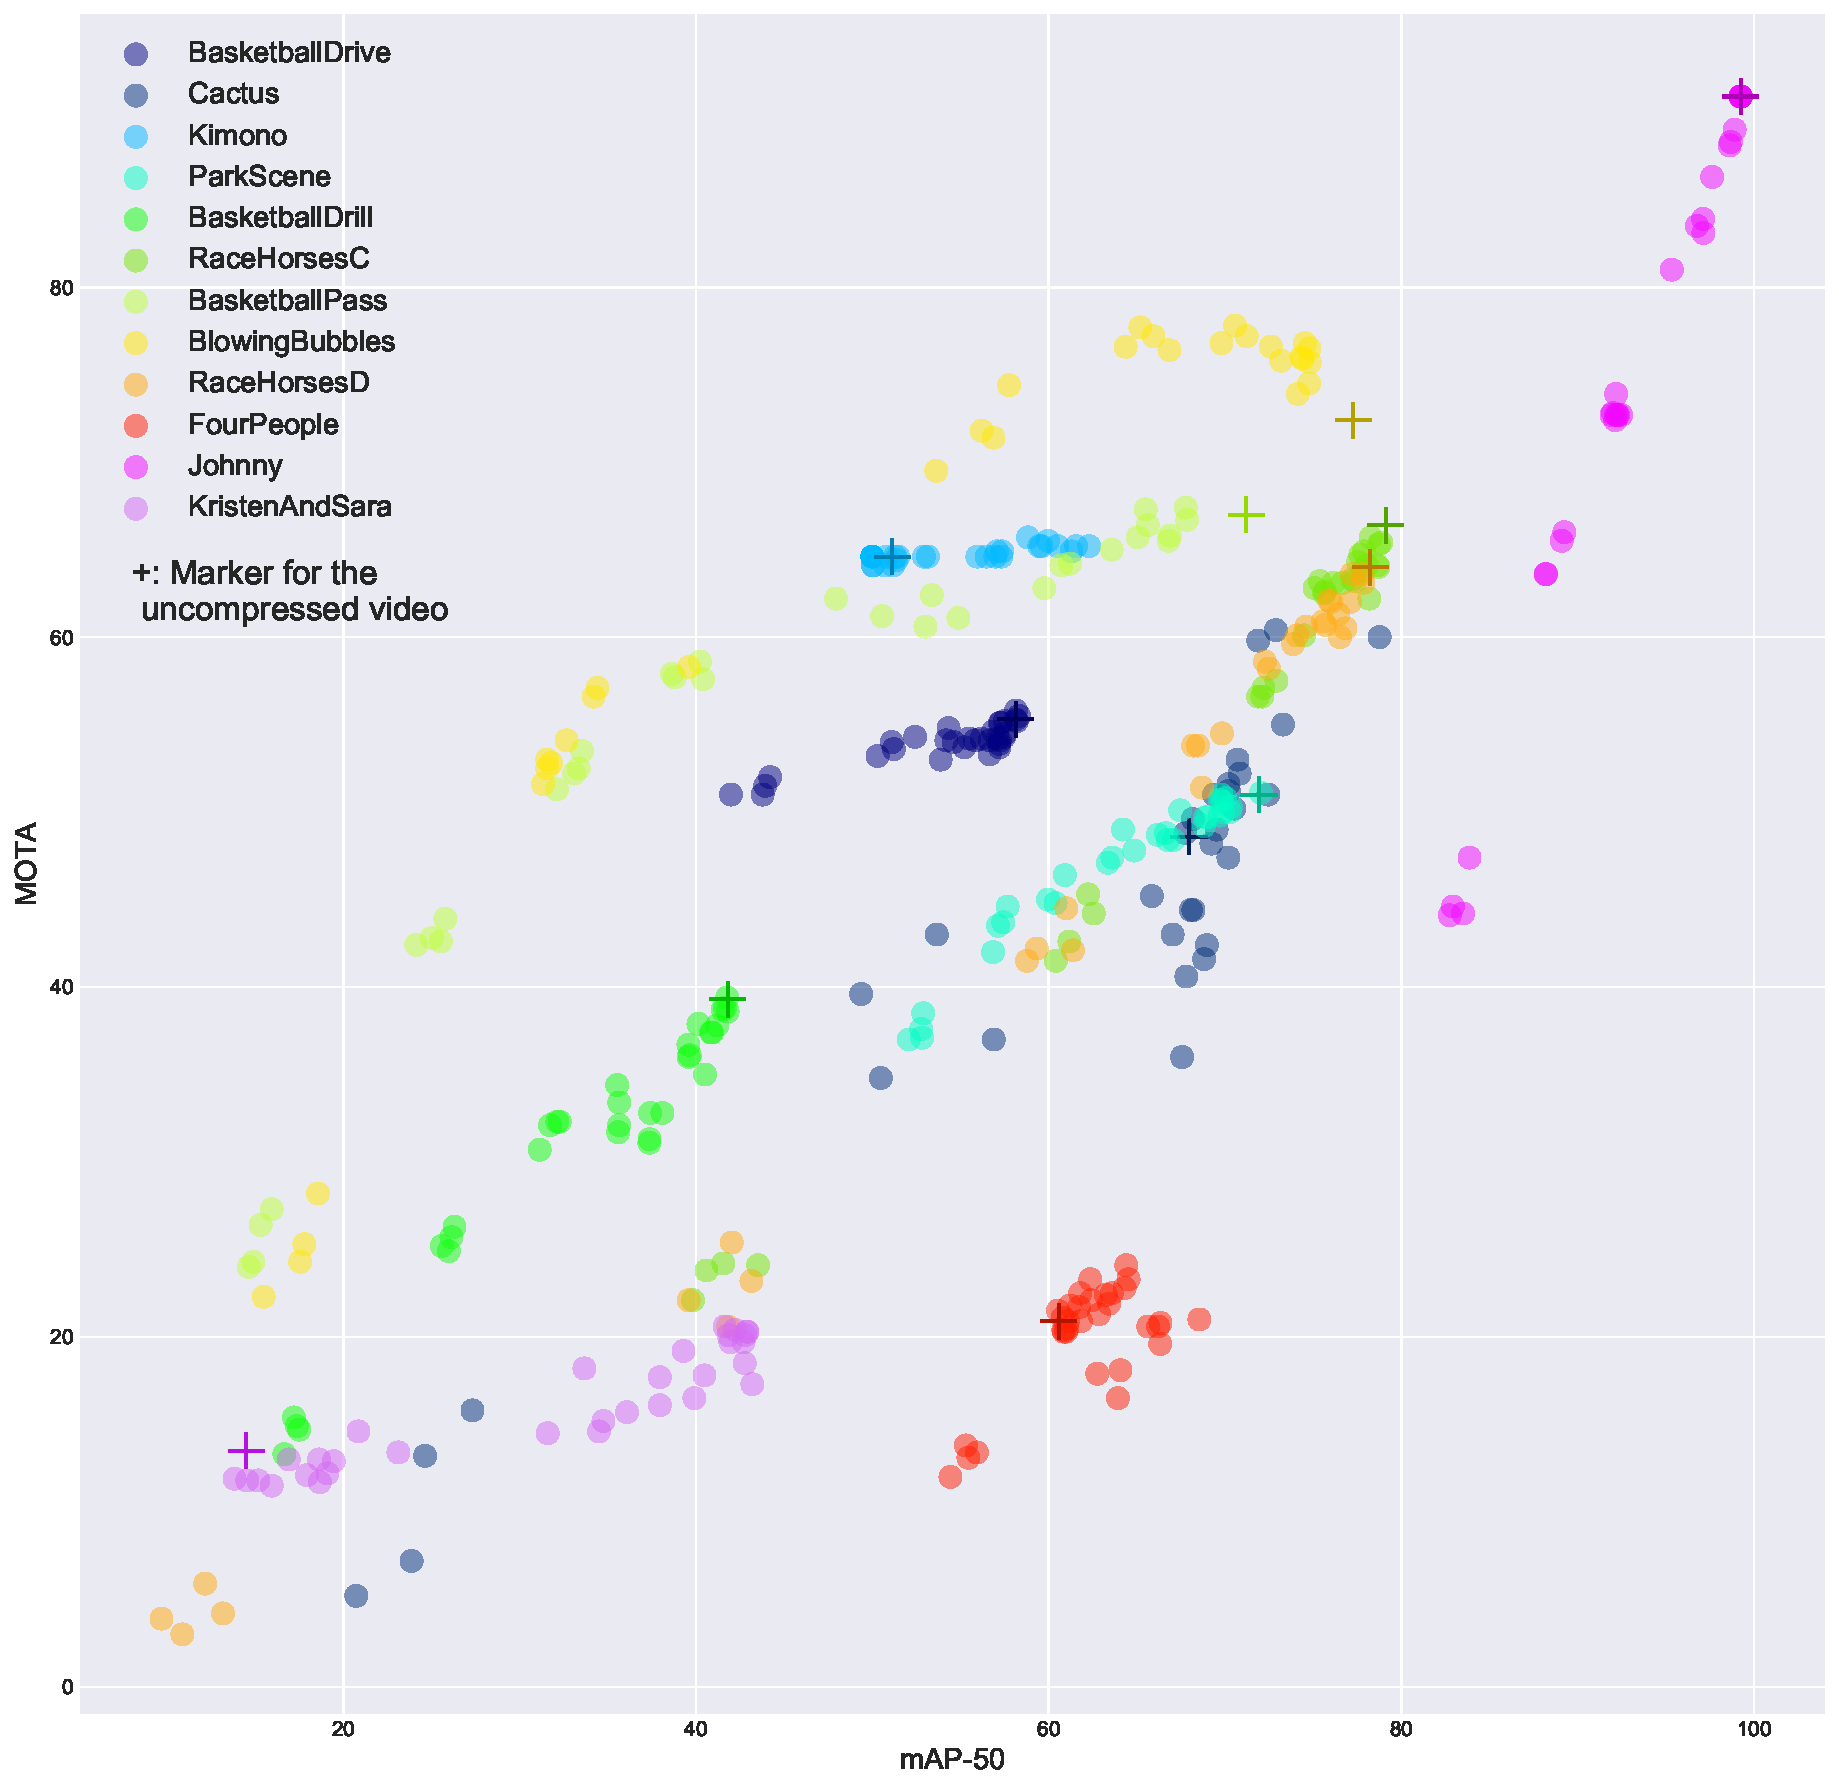
\includegraphics[width=0.8\linewidth]{img/MOTA_vs_mAP50.pdf}
  \caption[Scatter plot of MOTA vs. mAP-50 across all video sequences]
  {Scatter plot of MOTA vs. mAP-50 across all video sequence.}
  \label{fig:MOTA_vs_mAP50}
\end{figure}
This figure illustrates each scatter plot of video sequence colored differently, and "+" indicates uncompressed sequences. It is trivial from this scatter plot that the detection performance impacts the tracking performance because the higher the mAP-50 score, the higher the MOTA score is. As we are analyzing the relation between the two variables MOTA and mAP-50, we computed the Pearson correlation coefficient and obtained as 0.703. This value explains that the two variables mAP-50 and MOTA are positively related. To examine more carefully for each video sequence, from Figure \ref{fig:MOTA_vs_mAP50}, we can see that not all the sequences look linear. For example, RaceHorsesD shows a linear relationship but BasketballPass shows a non-linear relationship between MOTA and mAP-50, as shown in Figure \ref{fig:MOTA_vs_mAP50_example}. The similar cases for the non-linear outcome can be observed in other sequences as well. 
\begin{figure}[!tb]
  \centering
  \begin{subfigure}[b]{.5\textwidth}
    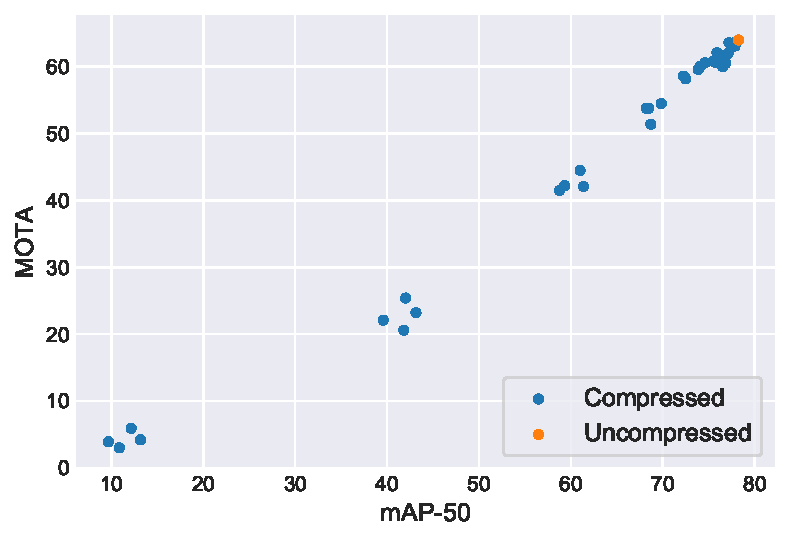
\includegraphics[width=\textwidth]{img/MOTA_vs_mAP50_RaceHorsesD.pdf}
    \caption{MOTA vs. mAP-50 scatter plot for RaceHorsesD}
    \label{fig:MOTA_vs_mAP50_RaceHorsesD}
  \end{subfigure}%
  \begin{subfigure}[b]{.5\textwidth}
    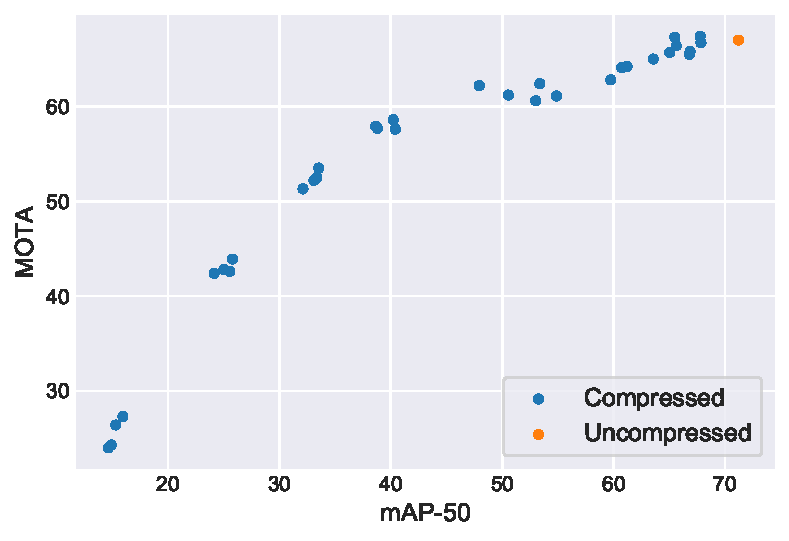
\includegraphics[width=\textwidth]{img/MOTA_vs_mAP50_BasketballPass.pdf}
    \caption{MOTA vs. mAP-50 scatter plot for BasketballPass}
    \label{fig:MOTA_vs_mAP50_BasketballPass}
  \end{subfigure}
  \caption[Linear and non-linear cases of scatter plots of MOTA and mAP-50]{%
    Linear and non-linear cases of scatter plots of MOTA and mAP-50.%
  }
  \label{fig:MOTA_vs_mAP50_example}
\end{figure}
The non-linear cases of result indicate that some factors could contribute to the concave down of the curve as an example shown in Figure \ref{fig:MOTA_vs_mAP50_BasketballPass}. Although we tested the parameters QP and MSR, there are other possible factors that we did not experiment with, for example, size of the bounding boxes and parameters in Kalman filter framework. The more thorough analysis will need to be conducted to identify such factors as a future study.